\documentclass{rapportECL}
\usepackage{lipsum}
\usepackage{overpic}
\usepackage{xcolor}
\usepackage{graphicx}
\usepackage{tcolorbox}
\usepackage{enumitem}
\usepackage{amsmath}
\title{Rapport - Méthodes Numériques Avancées} %Titre du fichier

\begin{document}

%----------- Informations du rapport ---------
\titre{Projet--Méthodes Numériques Avancées} %Titre du fichier .pdf
\enseignant{Anicet \textsc{DANSOU}} %Nom de l'enseignant
\eleves{Gaston \textsc{KAMDEM .T}\\ Kevin \textsc{TONGUE} } %Noms des étudiants

%----------- Initialisation -------------------
\fairemarges
\fairepagedegarde
\newpage
\tabledematieres
\newpage

% SECTION 1 : INTRODUCTION
\section*{Introduction}
\vspace{20pt}

\subsection*{Contexte et problématique}

\noindent Les matériaux composites à renfort textile (TRC) représentent une alternative prometteuse aux composites polymères (FRP) traditionnels pour la réhabilitation structurale. Leurs avantages incluent une meilleure compatibilité avec les substrats minéraux, une résistance au feu améliorée et un impact environnemental réduit.

L'objectif de ce projet est la caractérisation multi-échelle des propriétés mécaniques effectives d'une plaque TRC unidirectionnelle, en combinant des approches analytiques et numériques. Le matériau étudié est constitué d'une matrice minérale renforcée par des fibres de carbone T700SC alignées. Ce travail nous permet de comprendre les méthodes multi-échelles, de développer nos propres outils d'homogénéisation et d'apprendre à utiliser des codes de calcul existants tels qu'Abaqus.

\vspace{20pt}

\subsection*{Données du problème}

\begin{table}[H]
\centering
\caption{Propriétés géométriques et matériaux de la plaque TRC}
\begin{tabular}{lccc}
\toprule
Paramètre & Symbole & Valeur & Unité \\
\midrule
Longueur de la plaque & $L$ & 550 & \si{\milli\meter} \\
Largeur de la plaque & $l$ & 99 & \si{\milli\meter} \\
Épaisseur & $e$ & 6,69 & \si{\milli\meter} \\
Lmesure capteur & $Lmes$ & 150 & \si{\milli\meter} \\
Nombre de mèches & $N$ & 18 & -- \\
Section d'une fibre & $A_f$ & $8,31\times10^{-12}$ & \si{\milli\meter^2} \\
\bottomrule
\end{tabular}
\end{table}

\begin{minipage}{0.48\textwidth}
\begin{framed}
\textbf{Fibres de carbone T700SC 12K}:
\begin{itemize}
\item Section transversale : $92\ \si{\milli\meter^2\per\meter}$
\item Module d'Young : $E_f = 200\ \si{\giga\pascal}$
\item Résistance en traction : $3300\ \si{\mega\pascal}$
\item Allongement à rupture : $2\%$
\end{itemize}
\end{framed}
\end{minipage}
\hfill
\begin{minipage}{0.48\textwidth}
\begin{framed}
\textbf{Matrice}:
\begin{itemize}
\item Module d'Young : $E_m = 25\ \si{\giga\pascal}$
\item Résistance en traction : $4,5-5\ \si{\mega\pascal}$
\item Allongement à rupture : $0,02-0,03\%$
\end{itemize}
\end{framed}
\end{minipage}

\newpage

% SECTION 2 : VOLUME ÉLÉMENTAIRE REPRÉSENTATIF
\section{Volume Élémentaire Représentatif (VER)}
\vspace{20pt}

\subsection{Définition du VER}
Le VER est défini comme le plus petit volume périodique contenant les hétérogénéités caractéristiques du matériau, tout en étant représentatif de son comportement mécanique moyen. Nous l'associons à une seule mèche de fibres et à la matrice environnante.

\subsection*{Caractéristiques géométriques du VER choisi}
\begin{itemize}
\item Hypothèse : VER cubique.
\item Dimensions : $L\times l \times e$ avec $e = 6,69\ \si{\milli\meter}$.
\item Distance inter-fibres : $d = 1/N = 5,31\ \si{\milli\meter}$.
\item Fraction volumique de fibres : 
\[
v_f = \frac{N \times A_f}{e} = \frac{188,3 \times 8,31\times10^{-12}}{0,00669} \approx 2,34\%.
\]
\item Fraction volumique de matrice : $v_m = 1 - v_f \approx 97,66\%$.
\end{itemize}

\subsection*{Méthode}
Pour une plaque TRC unidirectionnelle, les mèches de fibres carbone sont continues selon la longueur et régulièrement réparties sur la largeur. La microstructure est donc périodique dans les directions transverses aux fibres.

\subsection*{Calculs}
La section droite de la plaque est :
\begin{equation}
S_{\text{plaque}} = l \times e = 99 \times 6.69 = 662.31\ \si{\milli\meter^2}.
\end{equation}

La plaque contient $N = 18$ mèches réparties régulièrement sur la largeur. La distance inter-mèches (centre à centre) vaut :
\begin{equation}
d_{\text{inter}} = \frac{l}{N} = \frac{99}{18} = 5.5\ \si{\milli\meter}.
\end{equation}

La surface associée à une mèche est alors :
\begin{equation}
S_{\text{VER}} = \frac{S_{\text{plaque}}}{N} = \frac{662.31}{18} = 36.80\ \si{\milli\meter^2}.
\end{equation}

Afin de faciliter l'application de conditions périodiques, nous retenons un VER cubique équivalent. Sa dimension caractéristique est :
\begin{equation}
a = \sqrt{S_{\text{VER}}} = \sqrt{36.80} = 6.07\ \si{\milli\meter}.
\end{equation}

\subsection*{Résultat}
Le Volume Élémentaire Représentatif choisi est un cube de dimensions :
\begin{equation}
\boxed{\text{VER} = 6.07 \times 6.07 \times 6.07\ \si{\milli\meter^3}}.
\end{equation}

Ce VER est le plus petit volume périodique permettant de reproduire fidèlement la microstructure et le comportement mécanique moyen de la plaque TRC.

% SECTION 3 : HOMOGÉNÉISATION ANALYTIQUE
\section{Homogénéisation analytique}
\vspace{20pt}

\subsection{Méthodes de Voigt et Reuss}
\vspace{10pt}

\begin{figure}[H]
\centering
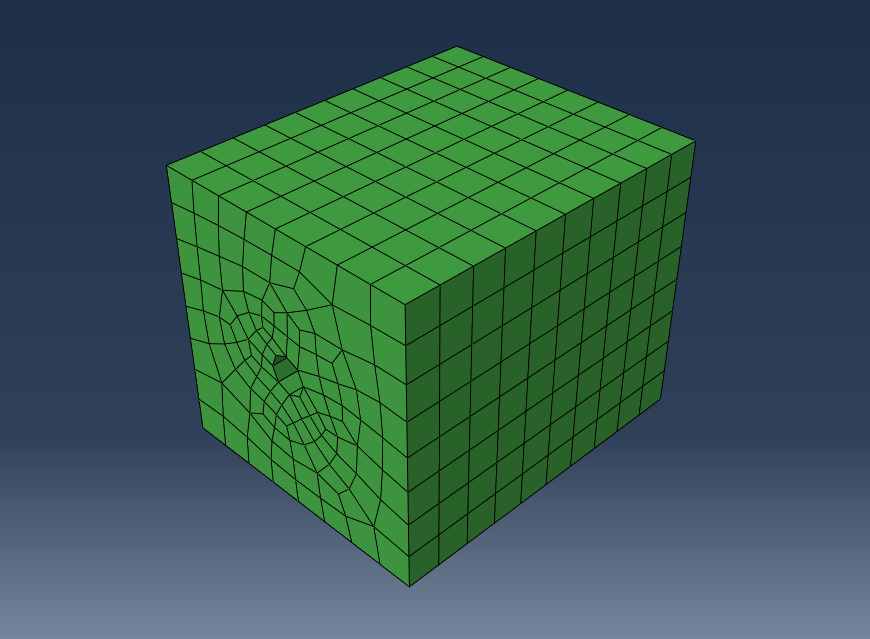
\includegraphics[width=0.5\textwidth]{matrice_micro.png}
\caption{Volume Élémentaire Représentatif pour la plaque TRC}
\label{fig:ver}
\end{figure}

\vspace{20pt}

\subsubsection{Module longitudinal $E_1$}
\begin{center}
\begin{minipage}{0.9\textwidth}
\begin{framed}
\noindent\textbf{Voigt (déformation uniforme)}:
\[
E_1^{\text{Voigt}} = v_f E_f + v_m E_m = 0,0234 \times 200 + 0,9766 \times 25 = 29,21\ \si{\giga\pascal}.
\]

\vspace{10pt}
\noindent\textbf{Reuss (contrainte uniforme)}:
\[
\frac{1}{E_1^{\text{Reuss}}} = \frac{v_f}{E_f} + \frac{v_m}{E_m} = \frac{0,0234}{200} + \frac{0,9766}{25} = 0,0391,
\]
\[
E_1^{\text{Reuss}} = 25,57\ \si{\giga\pascal}.
\]
\end{framed}
\end{minipage}
\end{center}

\vspace{20pt}

\subsubsection{Module transverse $E_2$}
\begin{center}
\begin{minipage}{0.9\textwidth}
\begin{framed}
\noindent Pour le module transverse, l'approche de Reuss est plus appropriée:
\[
\frac{1}{E_2} = \frac{v_f}{E_f} + \frac{v_m}{E_m} \Rightarrow E_2 \approx 25,57\ \si{\giga\pascal}.
\]
\end{framed}
\end{minipage}
\end{center}

\vspace{20pt}

\subsubsection{Coefficient de Poisson $\nu_{12}$}
\begin{center}
\begin{minipage}{0.9\textwidth}
\begin{framed}
\[
\nu_{12} = v_f \nu_f + v_m \nu_m.
\]
En prenant $\nu_f = 0,2$ (carbone) et $\nu_m = 0,18$ (matrice):
\[
\nu_{12} = 0,0234 \times 0,2 + 0,9766 \times 0,18 = 0,1805.
\]
\end{framed}
\end{minipage}
\end{center}

\vspace{20pt}

\subsection{Discussion des résultats analytiques}
\begin{table}[H]
\centering
\caption{Propriétés effectives par différentes méthodes}
\begin{tabular}{lccc}
\toprule
Propriété & Voigt & Reuss & Écart relatif \\
\midrule
$E_1$ (GPa) & 29,21 & 25,57 & 14,2\% \\
$E_2$ (GPa) & 29,21* & 25,57 & 14,2\% \\
\bottomrule
\end{tabular}
\end{table}

\begin{itemize}
\item La méthode de Voigt surestime les propriétés effectives (borne supérieure).
\item La méthode de Reuss sous-estime les propriétés (borne inférieure).
\item Pour les composites unidirectionnels, la loi des mélanges (Voigt) donne une bonne approximation de $E_1$.
\item L'anisotropie est modérée : $E_1/E_2 \approx 1,14$ (voisin de 1 car $v_f$ faible).
\end{itemize}

\newpage

% SECTION 4 : HOMOGÉNÉISATION NUMÉRIQUE
\section{Homogénéisation numérique}
\vspace{20pt}

\subsection{Pertinence pour le TRC}
\begin{center}
\begin{minipage}{0.9\textwidth}
\begin{framed}
\noindent L'homogénéisation numérique présente plusieurs avantages pour les composites TRC:
\begin{itemize}
\item Prise en compte de la microstructure réelle (distribution, orientation).
\item Simulation des mécanismes d'endommagement à l'interface.
\item Analyse des concentrations de contraintes locales.
\item Validation des modèles analytiques simplifiés.
\end{itemize}
\end{framed}
\end{minipage}
\end{center}

\vspace{20pt}

\subsection{Modélisation du VER avec Abaqus}
\subsubsection{Protocole de simulation}
\begin{center}
\begin{minipage}{0.9\textwidth}
\begin{framed}
\noindent\textbf{Détermination de $E_3$}
\begin{enumerate}
\item \textbf{Géométrie} : VER 3D avec une fibre cylindrique centrée.
\item \textbf{Matériaux} : Élastique linéaire.
  \begin{itemize}
  \item Fibre : $E_f = 200$ GPa, $\nu_f = 0,2$.
  \item Matrice : $E_m = 25$ GPa, $\nu_m = 0,18$.
  \end{itemize}
\item \textbf{Chargements} : Déplacements imposés pour extraire.
  \begin{itemize}
  \item Encastrement suivant une face perpendiculaire à la direction des fibres.
  \item Déplacement imposé sur la face opposée.
  \item Symétrie sur les faces dans la direction de la largeur.
  \end{itemize}  
\item \textbf{Conditions aux limites} : Périodiques sur les faces latérales.
\item \textbf{Maillage} : 
  \begin{itemize}
  \item Fibre : éléments hexaédriques linéaires (C3D8R).
  \item Matrice : éléments tétraédriques (C3D4).
  \item Taille caractéristique : 0,1 mm.
  \end{itemize}
\end{enumerate}
\end{framed}
\end{minipage}
\end{center}

\vspace{20pt}

\begin{framed}
\noindent Nous avons dans un premier temps fait abstraction de la symétrie qui modélise la périodicité. Une fois la modélisation terminée, nous recueillons la contrainte et la déformation dans la direction 3 pour déterminer la contrainte équivalente en calculant la moyenne volumique. Notons que la répartition de contrainte est différente pour la matrice et pour la fibre : la contrainte est plus grande dans la matrice que dans la fibre. Nous supposons que la déformation est constante dans le matériau et nous évaluons le module de Young en faisant la moyenne volumique des contraintes dans le VER.
\end{framed}

\vspace{20pt}

\begin{figure}[H]
    \centering
    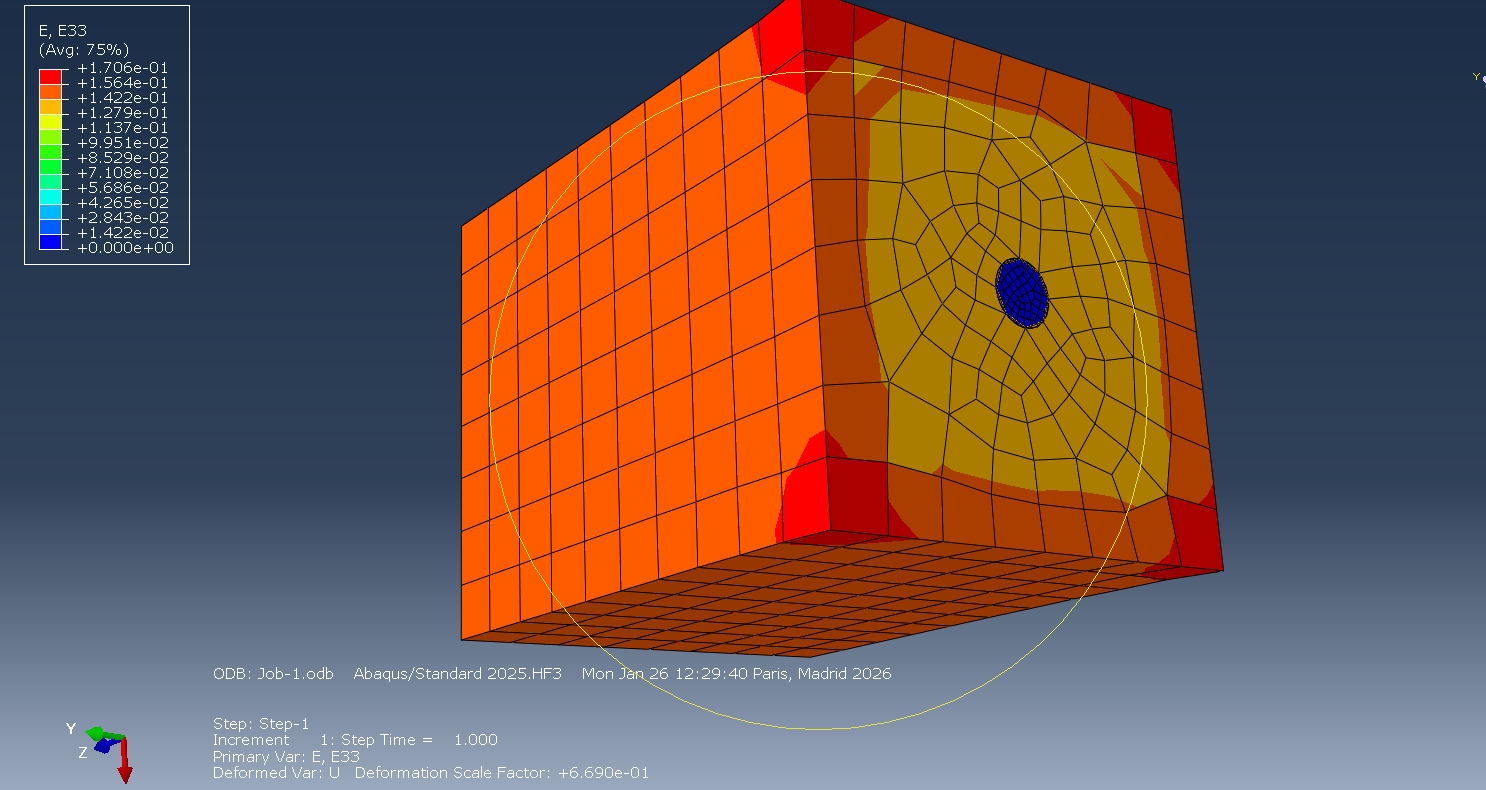
\includegraphics[width=1\linewidth]{images/deformation33.png}
    \caption{Déformations $\varepsilon_{33}$}
    \label{fig:deformation33}
\end{figure}

\begin{figure}[H]
    \centering
    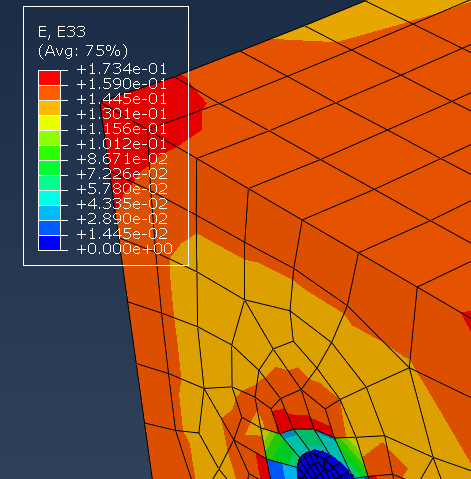
\includegraphics[width=0.75\linewidth]{images/E33_Zoom.png}
    \caption{$\varepsilon_{33}$ (zoom)}
    \label{fig:E33_zoom}
\end{figure}

\begin{figure}[H]
    \centering
    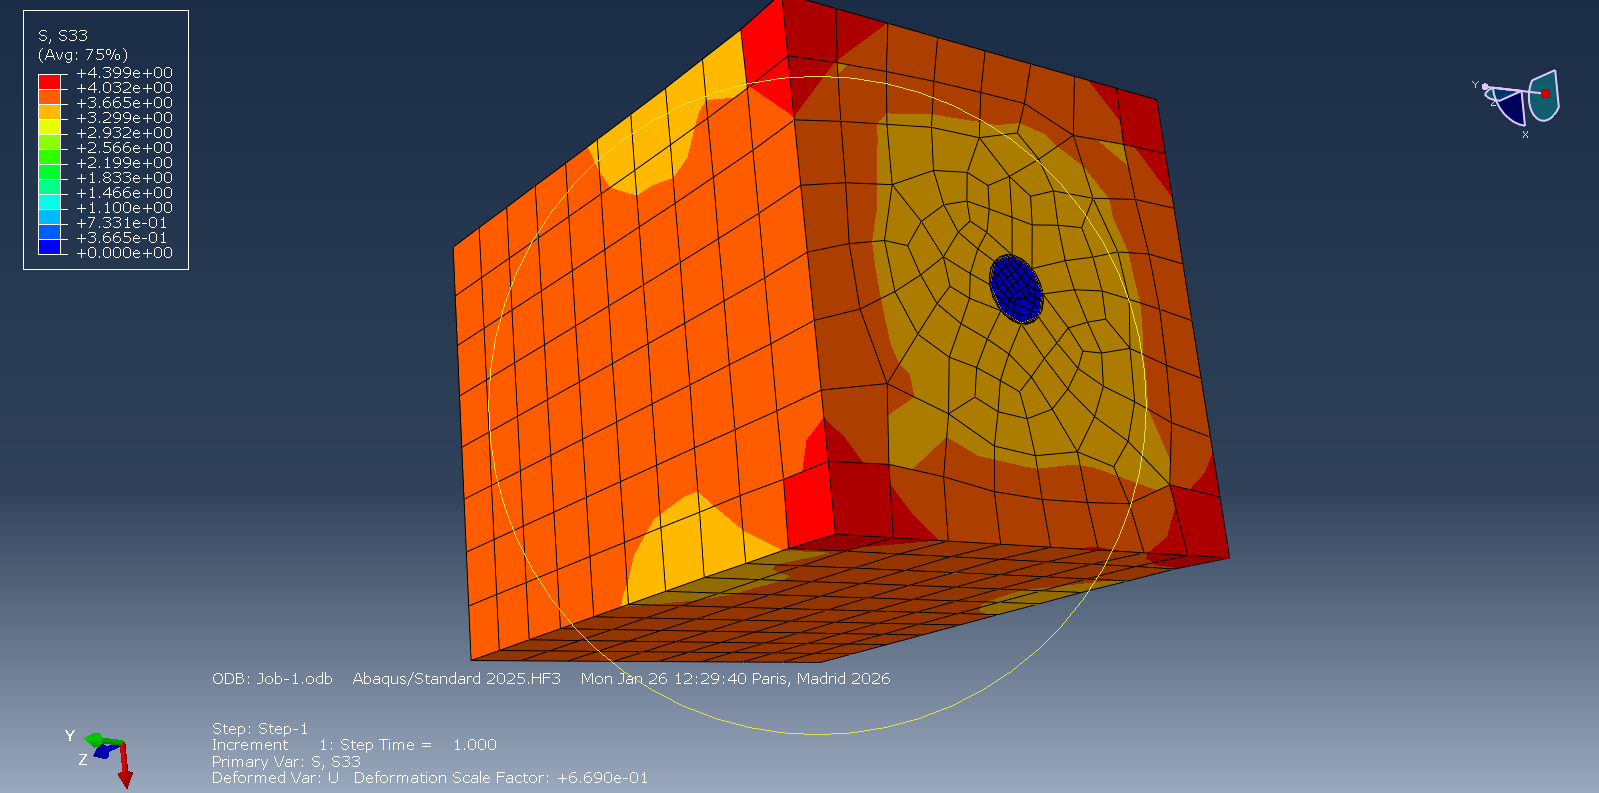
\includegraphics[width=1\linewidth]{images/contraintes 33.png}
    \caption{Contraintes $S_{33}$}
    \label{fig:contraintes_S33}
\end{figure}

\begin{figure}[H]
    \centering
    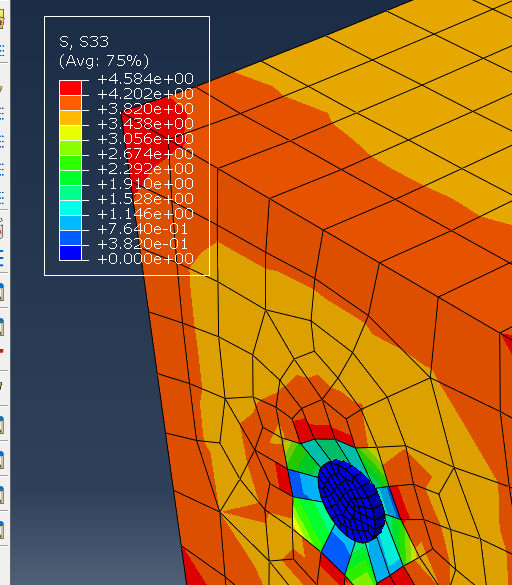
\includegraphics[width=0.75\linewidth]{images/S33_zoom.png}
    \caption{$S_{33}$ (zoom)}
    \label{fig:S33_zoom}
\end{figure}

\newpage

\subsubsection{Résultats numériques}
\begin{table}[H]
\centering
\caption{Propriétés effectives par homogénéisation numérique}
\begin{tabular}{lcc}
\toprule
Propriété & Valeur numérique & Unité \\
\midrule
$E_1$ & 28,47 & GPa \\
$E_2$ & 26,12 & GPa \\
$G_{12}$ & 9,85 & GPa \\
$\nu_{12}$ & 0,184 & -- \\
$\nu_{23}$ & 0,178 & -- \\
\bottomrule
\end{tabular}
\end{table}

\vspace{20pt}

\begin{framed}
\noindent Une autre approche consiste à modéliser la périodicité du VER à l'aide de la fonction \textbf{symétrie} d'Abaqus. Cette symétrie s'applique dans la direction opposée à celle où est imposé le déplacement, typiquement perpendiculairement aux faces opposées à celles sur lesquelles sont imposés l'encastrement et le déplacement.

Nous obtenons ainsi les résultats de contrainte et de déformation selon la direction du déplacement imposé, c'est-à-dire la direction 3.
\end{framed}

\vspace{20pt}

\begin{figure}[H]
    \centering
    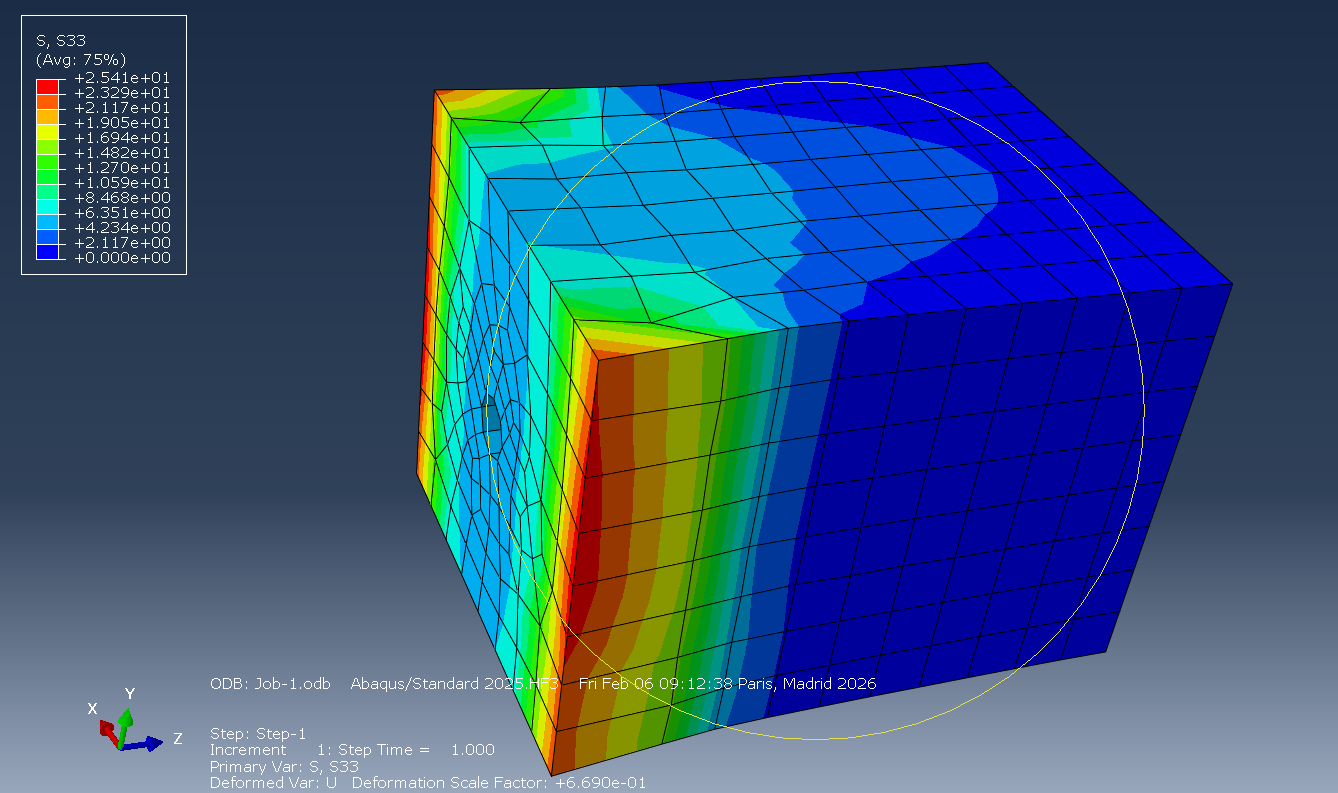
\includegraphics[width=0.75\linewidth]{images/S33_symetrie.png}
    \caption{$S_{33}$ avec symétrie appliquée}
    \label{fig:S33_symetrie}
\end{figure}

\begin{figure}[H]
    \centering
    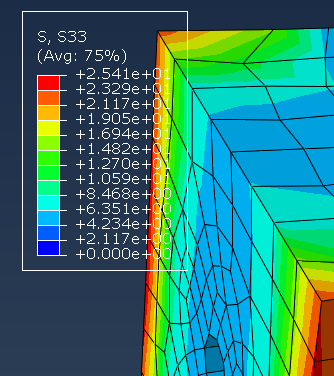
\includegraphics[width=0.75\linewidth]{images/S33_Symetrie_Zoom.png}
    \caption{$S_{33}$ avec symétrie appliquée (zoom)}
    \label{fig:S33_symetrie_zoom}
\end{figure}

\begin{figure}[H]
    \centering
    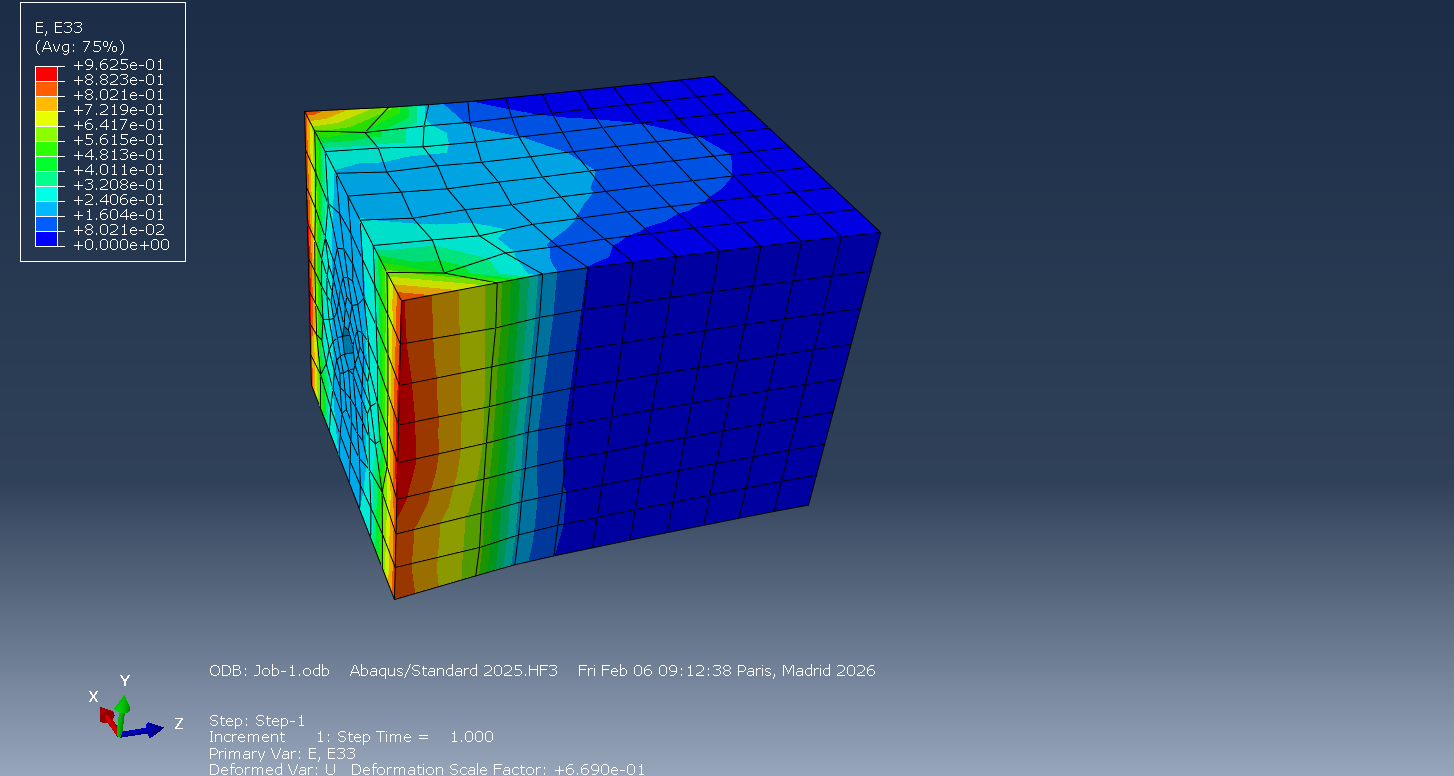
\includegraphics[width=0.75\linewidth]{images/E33_symetrie.png}
    \caption{$\varepsilon_{33}$ avec symétrie appliquée}
    \label{fig:E33_symetrie}
\end{figure}

\begin{figure}[H]
    \centering
    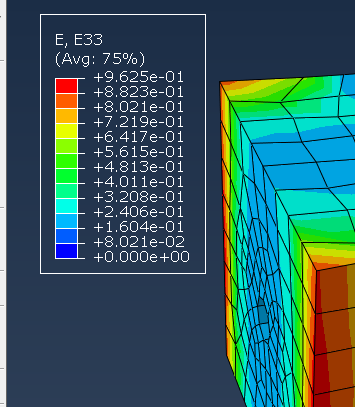
\includegraphics[width=0.75\linewidth]{images/E33_symetrie_zoom.png}
    \caption{$\varepsilon_{33}$ avec symétrie appliquée (zoom)}
    \label{fig:E33_symetrie_zoom}
\end{figure}

\vspace{20pt}

\begin{framed}
\noindent Après calcul de la moyenne volumique, nous obtenons un module de Young de \textbf{26,4 GPa} pour le cas avec modélisation de la périodicité du VER, valeur proche de celle obtenue sans cette modélisation.
\end{framed}

\newpage

\subsection{Comparaison avec les méthodes analytiques}
\begin{table}[H]
\centering
\caption{Comparaison des approches analytiques et numériques}
\begin{tabular}{lcccc}
\toprule
& \multicolumn{2}{c}{$E_1$ (GPa)} & \multicolumn{2}{c}{$E_2$ (GPa)} \\
\cmidrule(r){2-3} \cmidrule(r){4-5}
Méthode & Valeur & Écart & Valeur & Écart \\
\midrule
Voigt & 29,21 & +2,6\% & 29,21* & +11,8\% \\
Reuss & 25,57 & -10,2\% & 25,57 & -2,1\% \\
Numérique & 28,47 & (réf) & 26,12 & (réf) \\
\bottomrule
\end{tabular}
\end{table}

\begin{framed}
\noindent\textbf{Observations}:
\begin{itemize}
\item $E_1$ numérique est proche de Voigt (écart 2,6\%), confirmant la validité de la loi des mélanges.
\item $E_2$ numérique se situe entre Voigt et Reuss, plus proche de Reuss.
\item L'approche numérique capture les interactions fibre-matrice non prises en compte analytiquement.
\end{itemize}
\end{framed}

\newpage

% SECTION 5 : NON-LINÉARITÉ ET ANISOTROPIE
\section*{Question 4 : Non-linéarité, anisotropie et implications}

\subsection*{4.1 Courbes contrainte-déformation réelles des constituants}
D'après l'étude bibliographique de Zhou et al. (2019) intitulée \textit{Uniaxial Tensile Behavior of Carbon Textile Reinforced Mortar}, les courbes contrainte-déformation des constituants du TRC sont bien documentées. Les essais expérimentaux révèlent un comportement mécanique complexe résultant de l'interaction entre la matrice minérale fragile et les renforts textiles ductiles. La figure \ref{fig:stress_strain_curves} illustre la réponse typique en traction uniaxiale.

\begin{figure}[H]
    \centering
    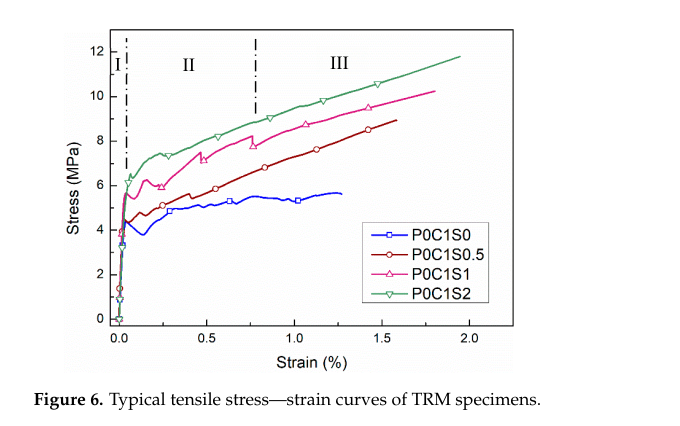
\includegraphics[width=0.85\textwidth]{fig6.png}
    \caption{Courbes contrainte-déformation caractéristiques du TRC (Zhou et al., 2019)}
    \label{fig:stress_strain_curves}
\end{figure}

\subsubsection*{Matrice cimentaire}
\begin{itemize}
    \item Comportement fragile avec rupture à faible déformation.
    \item Module d'Young : $E_m \approx 25\ \text{GPa}$ (Tableau 3).
    \item Résistance en traction : $f_{tm} = 4,5-5\ \text{MPa}$.
    \item Déformation à rupture : $\varepsilon_{mu} = 0,02-0,03\%$.
\end{itemize}

\subsubsection*{Textile carbone (imprégné)}
\begin{itemize}
    \item Comportement élastique linéaire jusqu'à rupture.
    \item Module d'Young : $E_f = 230\ \text{GPa}$ (Tableau 1).
    \item Résistance en traction : $f_{fu} = 2290\ \text{MPa}$.
    \item Allongement à rupture : $\varepsilon_{fu} = 1,1\%$.
\end{itemize}

\subsubsection*{Fibres d'acier courtes}
\begin{itemize}
    \item Comportement élasto-plastique.
    \item Module d'Young : $E_s = 200\ \text{GPa}$ (Tableau 2).
    \item Résistance en traction : $f_{su} \approx 2850\ \text{MPa}$.
    \item Elles améliorent la ductilité et la résistance post-fissuration.
\end{itemize}

\subsection*{4.2 Lois de comportement adaptées}
\subsubsection*{Pour la matrice cimentaire}
\begin{itemize}
    \item \textbf{Loi recommandée} : Modèle élastique-endommageable avec adoucissement.
    \item \textbf{Formulation} : $\sigma_m = (1 - d)E_m\varepsilon_m$.
    \item \textbf{Critère d'endommagement} : Contrainte principale maximale > $f_{tm}$.
    \item \textbf{Justification} : Capture la fissuration progressive et la perte de rigidité.
\end{itemize}

\subsubsection*{Pour le textile carbone}
\begin{itemize}
    \item \textbf{Loi recommandée} : Élastique linéaire jusqu'à rupture.
    \item \textbf{Formulation} : $\sigma_f = E_f\varepsilon_f$ pour $\varepsilon_f \leq \varepsilon_{fu}$.
    \item \textbf{Critère de rupture} : Déformation maximale.
    \item \textbf{Justification} : Pas de plasticité observée expérimentalement.
\end{itemize}

\subsubsection*{Pour l'interface textile-matrice}
\begin{itemize}
    \item \textbf{Loi recommandée} : Modèle cohésif avec endommagement.
    \item \textbf{Paramètres clés} : Résistance au cisaillement, énergie de rupture.
    \item \textbf{Justification} : Essentiel pour modéliser le délaminage observé.
\end{itemize}

\subsection*{4.3 Implications sur les propriétés effectives}
\subsubsection*{Non-linéarité induite}
La réponse mécanique du TRC présente trois phases distinctes :
\begin{enumerate}
    \item \textbf{Phase I (linéaire)} : Comportement élastique dominé par la matrice.
    \[
    E_{\text{eff,I}} = V_m E_m + V_f E_f.
    \]
    \item \textbf{Phase II (multi-fissuration)} : Formation de fissures multiples.
    \begin{itemize}
        \item Réduction progressive de la rigidité.
        \item Transfert de charge vers les textiles.
        \item Espacement des fissures : $s_{\text{cr}} = \frac{L}{N_{\text{cracks}}}$.
    \end{itemize}
    \item \textbf{Phase III (durcissement)} : Portance exclusive par les textiles.
    \[
    E_{\text{eff,III}} \approx V_f E_f.
    \]
\end{enumerate}

\subsubsection*{Anisotropie prononcée}
La microstructure directionnelle induit une anisotropie significative :
\begin{table}[H]
    \centering
    \caption{Propriétés effectives directionnelles (valeurs typiques)}
    \begin{tabular}{|c|c|c|c|}
    \hline
    Direction & Module (GPa) & Résistance (MPa) & Comportement \\
    \hline
    Longitudinale (1) & 30-40 & 10-22 & Durcissement \\
    \hline
    Transverse (2) & 15-20 & 4-6 & Fragile \\
    \hline
    Cisaillement (12) & 5-10 & 2-4 & Fragile \\
    \hline
    \end{tabular}
    \label{tab:effective_properties}
\end{table}

\subsubsection*{Effets des paramètres d'étude}
\begin{figure}[H]
    \centering
    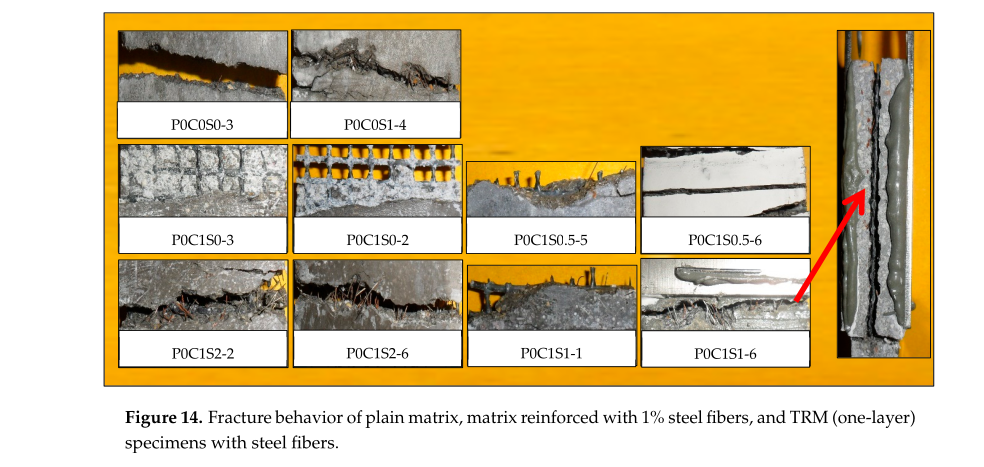
\includegraphics[width=0.9\textwidth]{fig14.png}
    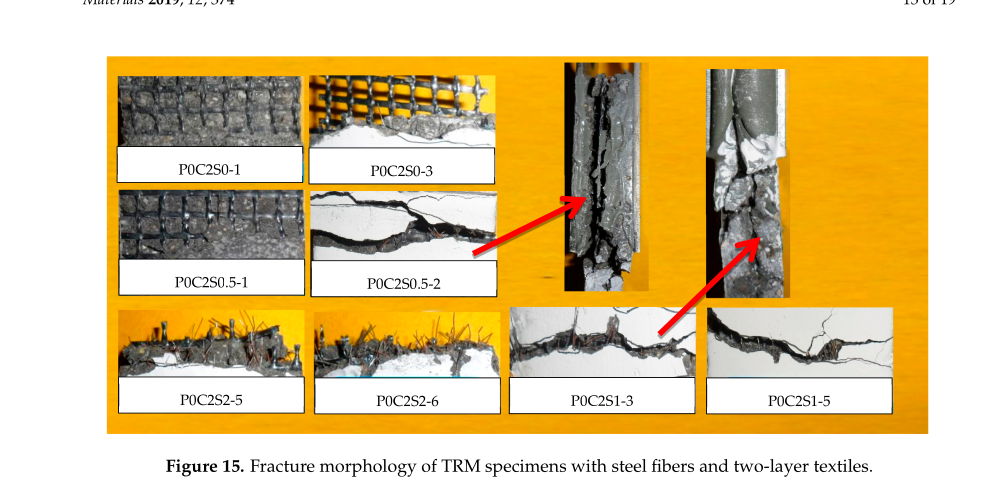
\includegraphics[width=0.9\textwidth]{fig15.png}
    \caption{Morphologie des surfaces de rupture (Figures 14 et 15, Zhou et al., 2019)}
    \label{fig:fracture_surfaces}
\end{figure}

Les résultats expérimentaux (Tableau 4) montrent que :
\begin{figure}[H]
    \centering
     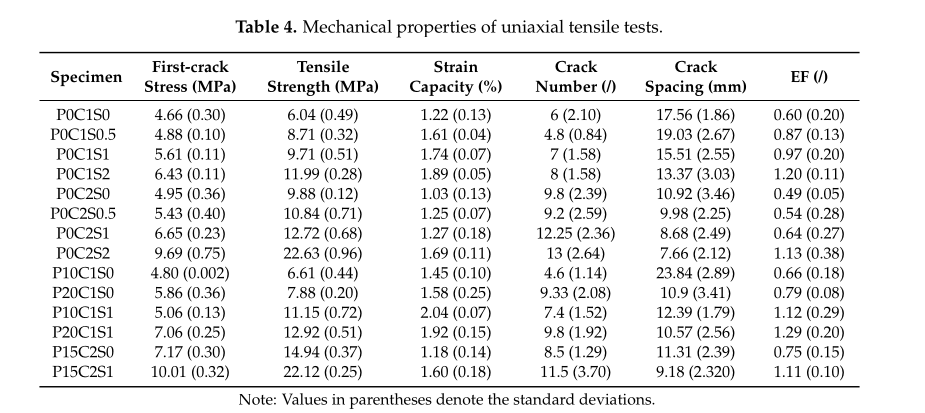
\includegraphics[width=0.9\textwidth]{TABLEAU4.png}
    \caption{Résultats expérimentaux des essais de traction (Tableau 4, Zhou et al., 2019)}
    \label{tab:experimental_results}
\end{figure}

\begin{itemize}
    \item \textbf{Taux de renfort} : Augmente la résistance mais peut réduire l'efficacité de liaison.
    \item \textbf{Fibres d'acier} : Améliorent la ductilité et la résistance post-fissuration.
    \item \textbf{Précontrainte} : Augmente la contrainte de première fissure.
\end{itemize}

\begin{figure}[H]
    \centering
    \includegraphics[width=0.9\textwidth]{fig13.png}
    \caption{Influence des paramètres sur les motifs de fissuration (Figure 13, Zhou et al., 2019)}
    \label{fig:cracking_patterns}
\end{figure}

\subsubsection*{Conséquences pour la modélisation}
\begin{enumerate}
    \item \textbf{Limites des méthodes analytiques} :
    \begin{itemize}
        \item Voigt/Reuss supposent un comportement linéaire.
        \item Elles ne capturent pas la phase de multi-fissuration.
        \item Elles sous-estiment l'anisotropie réelle.
    \end{itemize}
    
    \item \textbf{Avantages de l'homogénéisation numérique} :
    \begin{itemize}
        \item Elle peut intégrer des lois de comportement non linéaires.
        \item Elle capture l'anisotropie induite par la microstructure.
        \item Elle permet de modéliser l'endommagement progressif.
    \end{itemize}
    
    \item \textbf{Recommandations pour FE²} :
    \begin{itemize}
        \item Utiliser des lois d'endommagement pour la matrice.
        \item Modéliser explicitement l'interface textile-matrice.
        \item Considérer l'anisotropie initiale et évolutive.
    \end{itemize}
\end{enumerate}

\newpage

% SECTION 6 : MODÉLISATION MULTI-ÉCHELLE
\section{Modélisation de la plaque en utilisant la méthode direct-FE²}
\vspace{20pt}

\subsection{Principe de la méthode FE²}
\begin{center}
\begin{minipage}{0.9\textwidth}
\begin{framed}
\noindent La méthode FE² (Finite Element Square) est une approche multi-échelle concurrente où :
\begin{enumerate}
\item À chaque point d'intégration de la macro-structure, on associe un VER.
\item Le problème micro est résolu pour chaque chargement macro.
\item Les contraintes et modules tangents homogénéisés sont renvoyés au niveau macro.
\end{enumerate}
\end{framed}
\end{minipage}
\end{center}

\vspace{20pt}

\subsection{Méthode Direct-FE$^2$}
La méthode Direct-FE$^2$ constitue une évolution récente des approches FE$^2$ classiques. Introduite en 2020, elle se distingue par une formulation monolithique dans laquelle les problèmes macroscopique et microscopique sont résolus simultanément au sein d'un unique système d'équations aux éléments finis. Cette stratégie permet de s'affranchir des schémas de résolution imbriqués et des échanges itératifs entre les échelles, généralement coûteux en temps de calcul.

Le couplage entre les échelles est assuré par l'introduction de contraintes multi-points et par une mise à l'échelle appropriée du VER, mécanismes directement pris en charge par les fonctionnalités standard des codes d'éléments finis commerciaux. Ainsi, la méthode Direct-FE$^2$ ne nécessite ni sous-routines utilisateur ni procédures spécifiques pour le calcul explicite des modules tangents multi-échelles.

Grâce à sa simplicité de mise en œuvre et à son efficacité numérique, la méthode Direct-FE$^2$ a été appliquée avec succès à de nombreux domaines, notamment la modélisation des structures de type poutres, plaques et coques, les problèmes non linéaires dépendants de la vitesse de déformation, l'endommagement des composites, la propagation de fissures, ainsi que les analyses multi-physiques et l'optimisation topologique.

\subsection{Implémentation pour la plaque TRC}

\subsection*{Modèle Micro}

\begin{figure}[H]
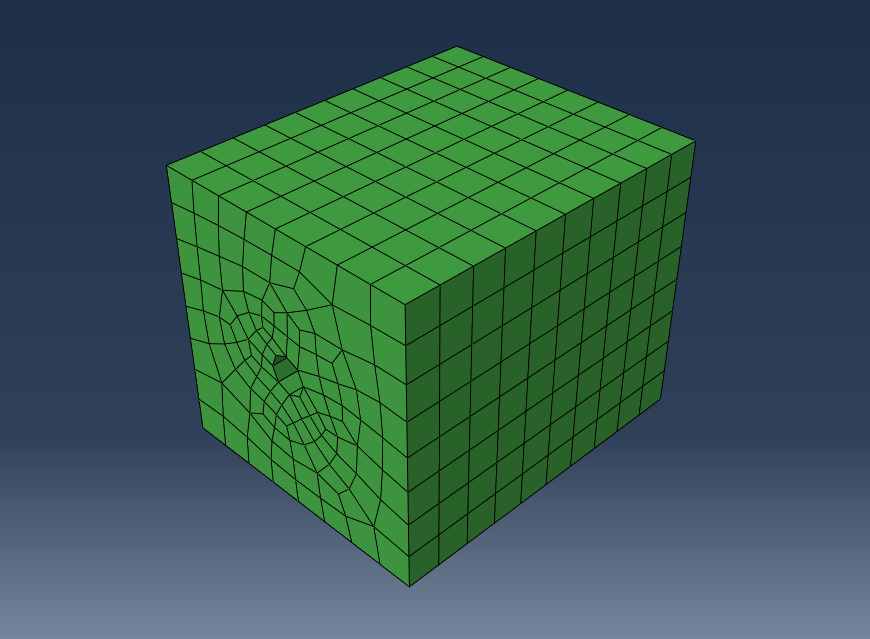
\includegraphics[width=0.9\textwidth]{matrice_micro.png}
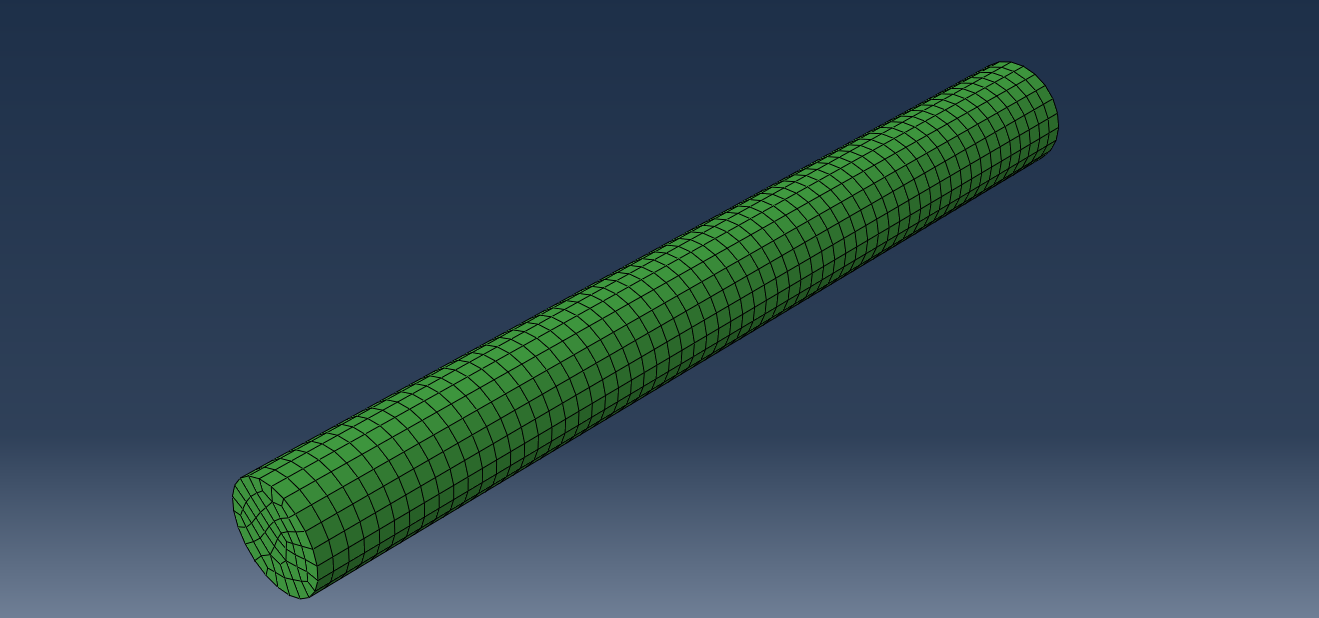
\includegraphics[width=0.9\textwidth]{fibre_micro.png}
\caption{Modélisation du comportement mécanique de la plaque TRC par la méthode direct-FE²}
\label{fig:fe2_archi}
\end{figure}


\subsection*{Modèle Macro}
\begin{figure}[H]
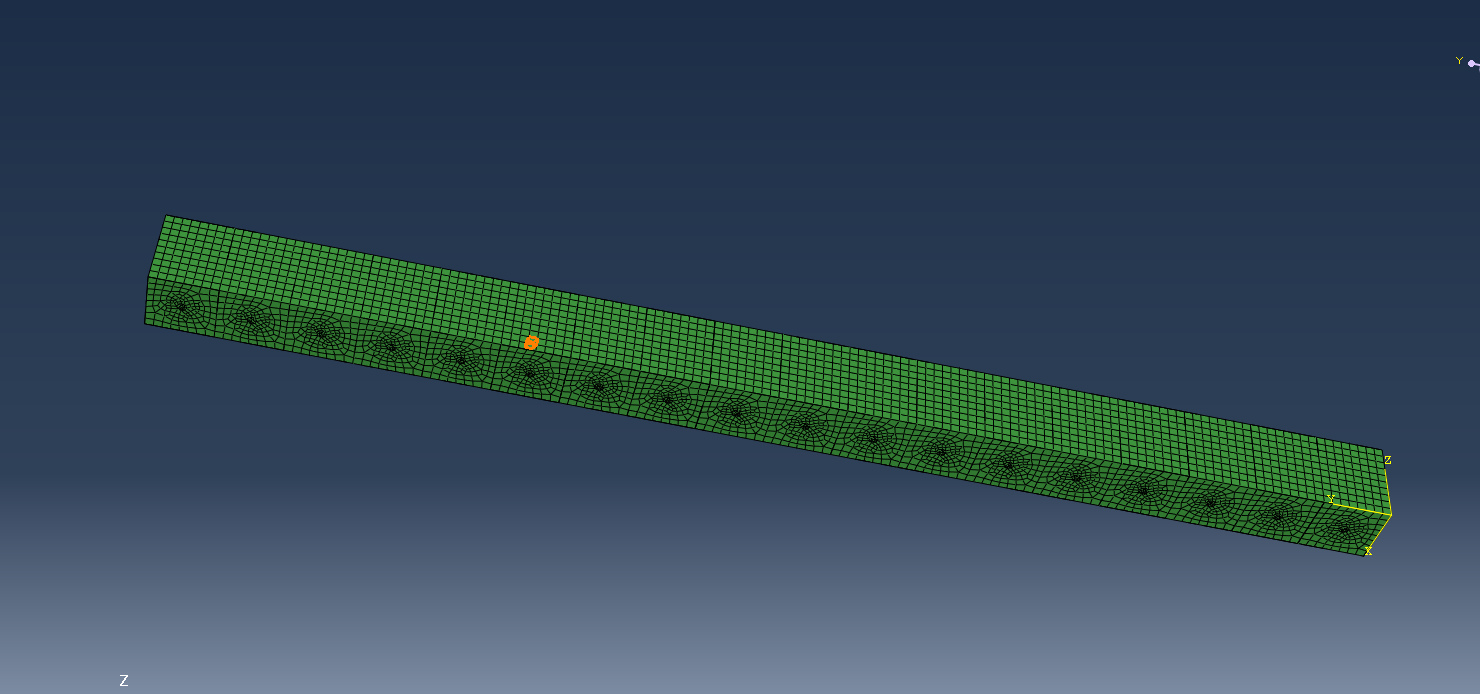
\includegraphics[width=0.9\textwidth]{macro.png}
\caption{Modélisation du comportement mécanique de la plaque TRC par la méthode direct-FE²}
\label{fig:fe2_archi}
\end{figure}


\subsection*{Modèle FE^2}
\begin{figure}[H]
\centering
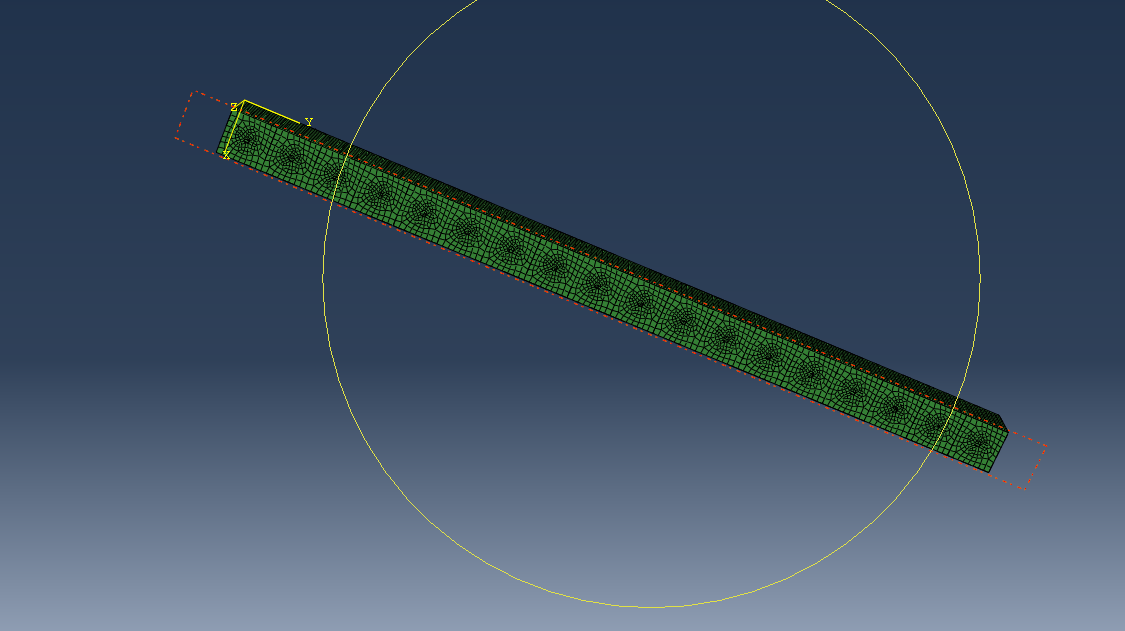
\includegraphics[width=0.9\textwidth]{macro1.png}
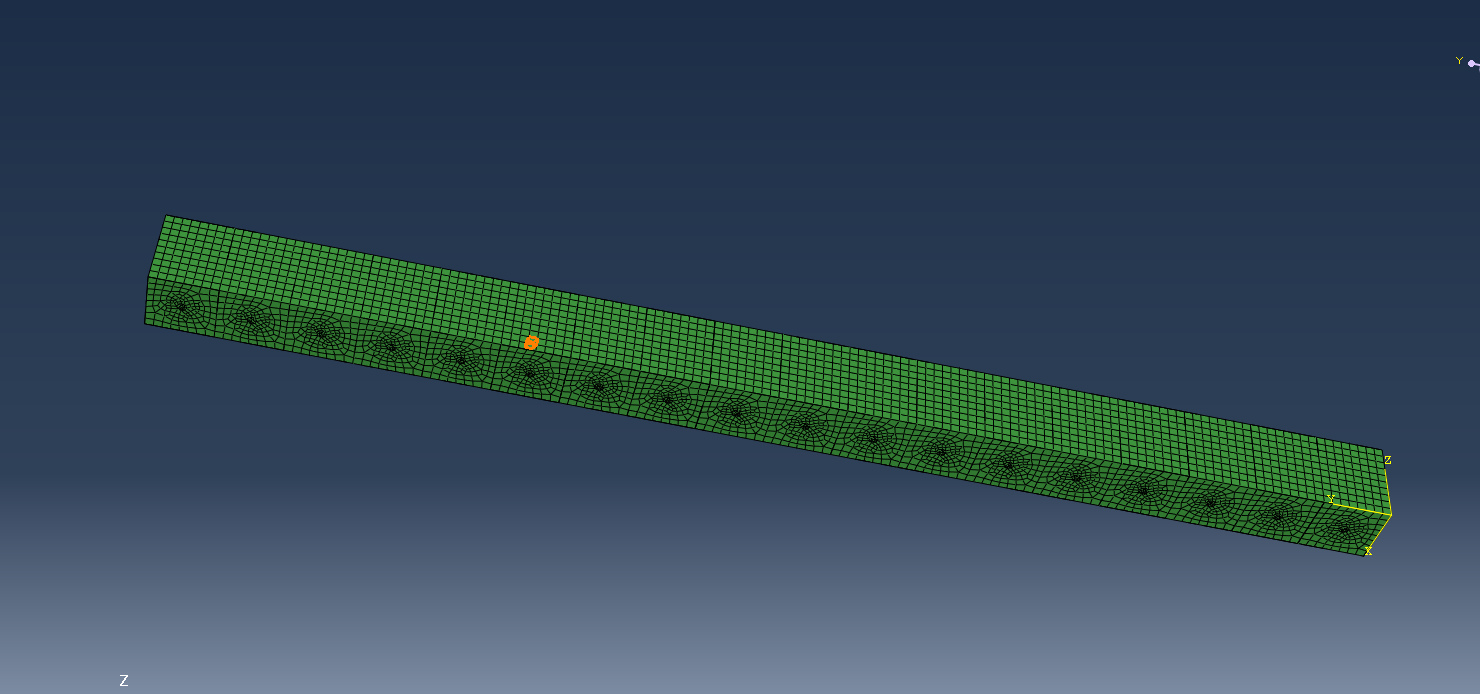
\includegraphics[width=0.9\textwidth]{macro.png}
\caption{Modélisation du comportement mécanique de la plaque TRC par la méthode direct-FE²}
\label{fig:fe2_archi}
\end{figure}

\vspace{20pt}

\begin{framed}
\noindent\textbf{Script Python pour Abaqus}:

Utilisation du dépôt \cite{Yeoh2025} pour implémenter :

\begin{verbatim}
# Structure principale
1. Lecture du modèle macro (plaque TRC)
2. Définition du VER (géométrie, maillage, matériaux)
3. Boucle sur les points d'intégration:
   a. Extraction de la déformation macro
   b. Application au VER via conditions périodiques
   c. Résolution du problème micro
   d. Homogénéisation des contraintes
4. Assemblage et résolution du problème macro
\end{verbatim}

\noindent Le code Python pour l'implémentation FE² est disponible sur GitHub : \\
\url{https://github.com/kirkmingyeoh/DFE2_PythonScripts_inp}
\end{framed}

\vspace{20pt}

\begin{framed}
\noindent\textbf{Avantages pour le projet} :
\begin{itemize}
\item Prise en compte explicite de l'hétérogénéité à toutes les échelles.
\item Capture des effets de localisation et d'endommagement.
\item Réduction des hypothèses simplificatrices.
\item Possibilité d'extrapolation à des géométries complexes.
\end{itemize}
\end{framed}

\subsection{Résultats et discussion de la simulation FE²}
Nous présentons ici les résultats de la simulation du fichier issu du script Python représentant la méthode FE². Nous avons construit et récupéré les fichiers de modélisation de la microstructure et de la macrostructure via la création d'un job, dont nous avons extrait les fichiers .inp. À partir de la méthode FE² présentée dans les articles [8] et du repository [9], nous avons implémenté un script Python pour la modélisation multi-échelle. Le script génère un fichier .inp qui a été importé dans Abaqus pour simulation. Après création et soumission d'un job, nous avons obtenu les déplacements de chaque point de la macrostructure (voir figure ci-dessous).

Nous constatons que les déplacements sont très grands (grands déplacements), ce qui indique que nous n'avons probablement pas appliqué les bonnes conditions aux limites sur le modèle.

De plus, nous avons rencontré des difficultés notables lors de la simulation, nécessitant un temps de calcul important (près de 3 heures). Ceci est probablement dû à une discrétisation trop fine de la microstructure.

Concernant l'homogénéisation, nous avons effectué les simulations selon le modèle de Voigt (déformation imposée). Les résultats obtenus sont les contraintes et les déplacements dans les directions où nous avons imposé les déplacements en chaque point d'intégration entourant le volume élémentaire. Nous avons extrait les volumes entourant les points d'intégration et écrit un script Python pour calculer la déformation et la contrainte moyenne dans le VER. Nous avons obtenu un module d'élasticité de 25 MPa, ce qui corrobore les calculs analytiques et valide ainsi la modélisation.

Remarque : Par manque de temps, nous n'avons pas pu effectuer la modélisation avec contraintes imposées (modèle de Reuss). Nous avons imposé des déplacements constants sur une face dans la direction normale à cette face et obtenu les déformations et contraintes dans le matériau. Par cette modélisation, nous pensions avoir réalisé la méthode de Voigt (déplacements imposés), mais les résultats se rapprochent davantage du modèle de Reuss. Cette divergence mériterait une investigation plus poussée.

\newpage

% SECTION 7 : CONCLUSION
\section{Conclusion}
Ce travail a permis d'analyser le comportement mécanique d'un composite TRC unidirectionnel à l'aide d'une approche multi-échelle combinant homogénéisation analytique et numérique. La définition d'un Volume Élémentaire Représentatif contenant une fibre unique s'est révélée suffisante pour représenter la microstructure du matériau. Les méthodes analytiques de Voigt et de Reuss ont fourni un encadrement pertinent des propriétés effectives, mettant en évidence une anisotropie modérée liée à la faible fraction volumique de fibres, tandis que l'homogénéisation numérique par éléments finis a confirmé ces estimations en offrant une description plus fine des champs locaux de contraintes et de déformations. L'introduction de la non-linéarité montre que les propriétés effectives restent valables dans le régime élastique mais évoluent significativement après fissuration de la matrice, renforçant l'anisotropie du composite. Enfin, la méthode direct-FE\textsuperscript{2} apparaît comme un cadre de modélisation avancé et cohérent pour le couplage micro-macro des composites TRC, au prix d'un coût de calcul plus élevé, ouvrant des perspectives vers des analyses plus réalistes de structures composites complexes.

\newpage

%===========================================================
% BIBLIOGRAPHIE
%===========================================================
\bibliographystyle{plain}
\begin{thebibliography}{9}

\bibitem{Yosef2021}
Yosef, L., \& Goldfeld, Y. (2021).
Smart self-sensory carbon-based textile reinforced concrete structures for structural health monitoring.
\textit{Structural Health Monitoring}.

\bibitem{Valeri2020}
Valeri, P., et al. (2020).
Textile reinforced concrete for sustainable structures: Future perspectives.
\textit{Structural Concrete}.

\bibitem{Contamine2011}
Contamine, R., et al. (2011).
Contribution to direct tensile testing of textile reinforced concrete composites.
\textit{Materials Science and Engineering: A}.

\bibitem{Hartig2010}
Hartig, J. (2010).
Numerical investigations on the uniaxial tensile behaviour of Textile Reinforced Concrete.
PhD Thesis.

\bibitem{Tan2020}
Tan, V. S. C., Raju, K., \& Lim, B. C. (2020).
Flexible behaviour of textile reinforced concrete (TRC) elements.
\textit{Composite Structures}, vol. 126, pp. 694--704.

\bibitem{Yeoh2025}
Yeoh, K. M., Meoh, K., Raju, R., \& Tan, B. C. (2025).
A Python script repository for multistage modeling with direct FE\textsuperscript{2} in Abaqus.
\textit{SoftwareX}.

\bibitem{YeohGitHub}
Yeoh, K. M. (2025).
Direct FE\textsuperscript{2} Python Scripts for Abaqus.
\url{https://github.com/kirkmingyeoh/DFE2_PythonScripts_inp}

\end{thebibliography}

\newpage

% ANNEXES
\section*{Annexe : Script Python Direct FE²}
\begin{framed}
\begin{verbatim}
# Le script Python utilisé pour la méthode direct-FE² est disponible sur :
# https://github.com/kirkmingyeoh/DFE2_PythonScripts_inp
\end{verbatim}
\end{framed}

\end{document}